\documentclass{szb-practice}

\title{Elsőrendű és szétválasztható DE}
\area{Differenciálegyenletek}
\subject{Matematika G3}
\subjectCode{BMETE94BG03}
\date{Utoljára frissítve: \today}
\docno{9}

\usepackage{siunitx}
\sisetup{locale = DE}

\usetikzlibrary{snakes}

\begin{document}
\maketitle

\subsection{Elméleti áttekintő}

\begin{definition}[Lipschitz-feltétel][nobreak]
  Az $f : \Reals^2 \rightarrow \Reals$ függvényre azt monjuk,
  hogy  a $D$ tartományon az $y$ változóra nézve kielégíti a
  Lipschitz-feltételt, ha $\exists M \in \Reals^+$, hogy
  $\forall$ $\left( x; y_1 \right)$ és $\left( x; y_2 \right)$ esetén
  $$
    \left| f(x; y_1) - f(x; y_2) \right| \leq M \left| y_1 - y_2 \right|.
  $$
\end{definition}

\begin{theorem}[Picard-Lindelöf-tétel][]
  Legyen $y' = f(x, y)$ adott és $D = I_1 \times I_2$, ahol $I_1$ és $I_2$ nyílt
  intervallumok, $\left( x_0 ; y_0 \right) \in D$. Tegyük fel hogy:
  \begin{itemize}
    \item $f$ mindkét változójában folytonos $D$-n,
    \item $f$ kielégíti a Lipschitz-feltételt az $y$
          változójára nézve.
  \end{itemize}
  Ekkor az $y' = f(x; y)$, $y(x_0) = y_0$ kezdeti feltétellel
  ellátott differenciálegyenletnek $\exists!$ megoldása, azaz
  $\exists \varepsilon > 0$, hogy $\varphi :
    \left( x_0 - \varepsilon; \; x_0 + \varepsilon \right)
    \rightarrow \Reals$-re teljesül, hogy $\varphi' (x)
    = f \left(x ; \varphi(x)\right)$ és
  $\forall x \in \left( x_0 - \varepsilon; \; x_0 + \varepsilon \right)$
  esetén $\varphi(x_0) = y_0$.
\end{theorem}

\begin{theorem}[Szukcesszív approximáció]
  Ha az $y' = f(x; y)$ differenciálegyenletben lévő $f$ függvényre teljesül,
  hogy $\left| x - x_0 \right| < a \leq \infty$ és $\left| y - y_0 \right| < b
    \leq \infty$ tartományon korlátos és folytonos, továbbá eleget tesz a
  Lipschitz-feltételnek, akkor a
  $$
    y_{n + 1}
    := \underbrace{y(x_0)}_{y_0}
    + \int_{x_0}^x f\left(
    t; y_{n}(t)
    \right) \dd t
  $$
  függvénysorozat $n \rightarrow \infty$ esetén az $y' = f(x; y)$, $y(x_0) =
    y_0$ differenciálegyenlet megoldásához konvergál az  $\left| x - x_0 \right|
    < \min \left\{ a; b/M \right\}$  intervallumon.
\end{theorem}

\begin{example}
  Oldjuk meg az $y'(x) = x + y(x)$, $y_0 = 0$ Cauchy-feladatot szukcesszív
  approximációval!

  \boxrule

  Az iteráció során használt összefüggés:
  $$
    y_{n + 1}
    = y_n + \int_{x_0}^x f\left( t; y_{n}(t) \right) \dd t
    = 0 + \int_0^x \left( t + y_n(t) \right) \dd t
    \text.
  $$
  Számítsuk ki az első pár iterációt:
  \begin{align*}
    y_0(x)  & = 0 \text,
    \\
    y_1(x)  & = \int_0^x \left( t + 0 \right) \dd t = \frac{x^2}{2} \text,
    \\
    y_2(x)  & = \int_0^x \left( t + \frac{t^2}{2} \right) \dd t
    = \frac{x^2}{2} + \frac{x^3}{6} \text,
    \\
    y_3 (x) & = \int_0^x \left( t + \frac{t^3}{2} \right) \dd t
    = \frac{x^2}{2} + \frac{x^3}{6} + \frac{x^4}{24} \text,
    \\
    y_4(x)  & = \int_0^x \left( t + \frac{t^4}{2} \right) \dd t
    = \frac{x^2}{2} + \frac{x^3}{6} + \frac{x^4}{24} + \frac{x^5}{120} \text,
    \\
            & \vdots
    \\
    y_n(x)  & = -1 -x + \underbrace{1 + x + \frac{x^2}{2} + \frac{x^3}{6} + \dots}_{\to e^x}
    = e^x - 1 - x
    \text.
  \end{align*}
\end{example}

\begin{definition}[Szeparábilis differenciálegyenlet megoldása]
  $$
    y' = f(x)g(y)
    \quad \Rightarrow \quad
    \int \frac{\dd y}{g(y)} = \int f(x) \dd x
  $$
\end{definition}

\begin{blueBox}[$y' = f(ax + by + c)$ típusú differenciálegyenlet megoldása]
  Éljünk az $f(u)$ helyettesítéssel, ahol $u(x) = ax + by + c$, ennek deriváltja
  pedig $u' = a + b y' = a + b f(u)$. Ekkor a differenciálegyenlet az alábbi
  alakra redukálódik:
  $$
    \frac{\dd u}{a + b f(u)} = \dd x
    \text,
  $$
  amelyet integrálással már meg tudunk oldani.
\end{blueBox}

\begin{example}[Adjuk meg az alábbi differenciálegyenlet általános megoldását:][nobreak]
  $$
    y' = \exp(2x + 3y - 1)
  $$
  \boxrule

  Éljünk az $u(x) = 2x + 3y - 1$ helyettesítéssel, ennek deriváltja
  $u' = 2 + 3y' = 2 + 3e^u$. A kapott differenciálegyenlet már integrálással
  megoldható:
  $$
    \int\frac{\dd u}{2 + 3e^u} = \int\dd x
    \quad\Rightarrow\quad
    \frac{1}{2} \ln \left( \frac{e^u}{2 + 3e^u} \right) = x + K
    \quad\Rightarrow\quad
    \frac{e^u}{2 + 3e^u} = C e^{2x}
    \text.
  $$
  Visszahelyettesítve $u$-t, majd átrendezve:
  $$
    \frac{e^{2x + 3y - 1}}{2 + 3e^{2x + 3y - 1}} = C e^{2x}
    \quad\Rightarrow\quad
    y = \frac13 \left( 1 + \ln \frac{C}{1 - Ce^{2x}} \right)
    \text.
  $$
\end{example}

\begin{blueBox}[\underline{Newton lehűlési törvénye}]
  A Newton-féle lehűlési törvény azt írja le, hogyan változik egy test
  hőmérséklete az időben, ha a környezetével hőcserében van. A modell feltevése,
  hogy a hőmérsékletváltozás sebessége arányos a test és a környezet
  hőmérsékletének különbségével. Ha a környezet hőmérséklete $x_k$, a test
  hőmérséklete pedig $x(t)$, akkor az arányosság miatt a következő
  differenciálegyenletet kapjuk:
  $$
    \quad \dot{x} = \alpha(x - x_k)
    \text.
  $$
  A differenciálegyenlet szétválaszható, így az alábbi megoldáshoz jutunk:
  \begin{gather*}
    \frac{\dd x}{x - x_k} = \alpha \dd t
    \quad \Rightarrow \quad
    x(t) = x_k + C \cdot e^{\alpha t}
    \text,
  \end{gather*}
  ahol $C$ a kezdeti feltételből határozható meg.
\end{blueBox}

\begin{blueBox}[\underline{Általános keverési feladat}]
  Az általános keverési feladat tipikusan olyan helyzetet modellez, amikor egy
  tartályban lévő oldat koncentrációja az időben változik, mivel az oldatba új
  anyag áramlik be, illetve ugyanakkor oldat hagyja el a tartályt. A mennyiségi
  változásokat a koncentráció ($p$), illetve az oldat mennyisége ($V$) írja le.
  Feltesszük, hogy a tartályban a keverés tökéletes, tehát a koncentráció minden
  pillanatban egyenletes a térfogat teljes terében.

  \vspace{1em}

  \begin{minipage}[c]{.5\textwidth}
    \centering
    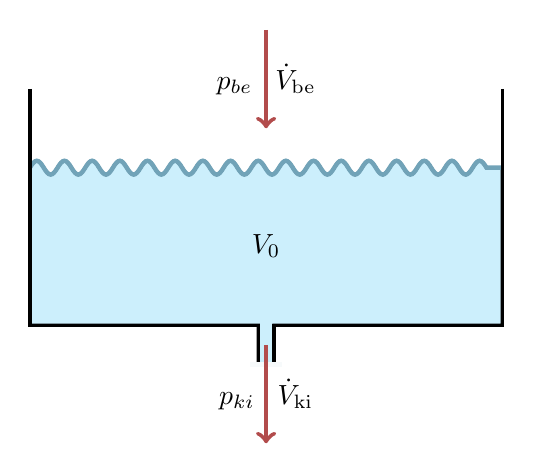
\begin{tikzpicture}
      \filldraw[snake=coil, segment aspect=0, very thick, cyan!40!gray, fill=cyan!20] (-3, 2)
      -- ++(6, 0)
      [snake=none, black, fill=cyan!20]-- ++(0,-2)
      -- ++(-2.9, 0)
      -- ++(0,-0.5)
      -- ++(-0.2, 0)
      -- ++(0,0.5)
      -- ++(-2.9, 0)
      -- ++(0, 2)
      ;
      \draw[snake=coil, segment aspect=0, ultra thick, cyan!40!gray] (-3,2) -- ++(6,0);

      \draw[very thick] (-3, 3) -- (-3, 0) -- (-0.1, 0) -- (-0.1, -0.5);
      \draw[very thick] (3, 3) -- (3, 0) -- (0.1, 0) -- (0.1, -0.5);

      \draw[cyan!40!gray!5!white, ultra thick] (0.2, -0.5) -- ++(-.4, 0);

      \draw[red!40!gray, ultra thick, -to] (0, 3.75) -- (0, 2.5)
      node [midway, black] {$p_{be} \;\;\; \dot{V}_\text{be}$};
      \draw[red!40!gray, ultra thick, -to] (0, -0.25) -- (0, -1.5)
      node [midway, black] {$p_{ki} \;\;\; \dot{V}_\text{ki}$};

      \node[] at (0, 1) {$V_0$};
    \end{tikzpicture}
  \end{minipage}\hfill
  \begin{minipage}[c]{.5\textwidth}
    Ha a bejövő és a kiáramló anyagmennyiség megegyezik
    ($\dot{V}_\text{be} = \dot{V}_\text{ki} = \dot{V}_\text{e} \in \Reals$),
    akkor:
    \begin{gather*}
      x_\text{be} = \dot{V}_\text{e} \cdot p_\text{be}
      \quad \quad \quad
      x_\text{ki}(t) = \frac{\dot{V}_\text{e}}{V_0} \; x(t)
      \\[2mm]
      \dot{x}(t) = x_\text{be} - x_\text{ki}(t)
      \\[2mm]
      \frac{\dd x}{x_\text{be} - x_\text{ki}(t)} = \dd t
    \end{gather*}

    Ha a bejövő és a kiáramló anyagmennyiség nem egyezik meg,
    azaz $\dot{V}_\text{be} \neq \dot{V}_\text{ki}$, ekkor:
    $$
      x_\text{ki}(t) = \frac{\dot{V}_\text{ki}}{V_0 + (\dot{V}_\text{be} - \dot{V}_\text{ki})t} \; x(t)
    $$
  \end{minipage}

  \vspace{1em}

  A keverési folyamat viselkedése mindkét esetben exponenciális közelítést mutat
  egy egyensúlyi koncentráció felé, hasonlóan a Newton-féle lehűlési törvényhez.
\end{blueBox}

\clearpage
\subsection{Feladatok}

\begin{enumerate}
  \item Adja meg az $y' = 3y^{2/3}$ differenciálegyenlet $y(0) = 0$ kezdeti
        feltétel melletti megoldását! Vizsgálja meg a megoldás egyértelműségét!

  \item Adja meg azt a tértartományt, ahol az $y' = x^2 + y^2$
        differenciálegyenlet megoldása egyértelmű!

  \item Adja meg azt a tértartományt, ahol az $y'' = y + 3 \sqrt{y} + e^{y'}$
        differenciálegyenlet megoldása egyértelmű!

  \item Számítsa ki az $y' = y$ differenciálegyenlet szukcesszív
        approximációjával kapott első négy közelítő függvényt, ha a kezdeti
        feltétel $y(0) = 1$!

  \item Számítsa ki az $y' = xy$ differenciálegyenlet szukcesszív
        approximációjával kapott első négy közelítő függvényt, ha a kezdeti
        feltétel $y(0) = 1$!

  \item Oldja meg a következő szétválasztható differenciálegyenleteket!
        \begin{alignat*}{9}
          a & ) \quad (2x + 1) y' - 3y = 0
          \text,                                                            \\
          b & ) \quad \sqrt{1 + x^2} \, y' - \sqrt{1 - y^2} = 0
          \text,                                                            \\
          c & ) \quad y' = \frac{1 - x - y}{2x - 2y - 3}
          \text,                                                            \\
          d & ) \quad xy' = y(1 + \ln x - \ln y)
          \text,                                                            \\
          e & ) \quad 2xyy' = x^2 + y^2
          \text,                                                            \\
          f & ) \quad y' = \frac{3x^2 + 4x + 2}{2y - 2}
          \text,
            & \qquad                                            & y(0) = -1
          \text,                                                            \\
          g & ) \quad xy' = x \cdot e^{\sfrac{y}{x}} + y
          \text,
            & \qquad                                            & y(1) = 0
          \text.
        \end{alignat*}

  \item Adja meg azon görbét, amelynek bármely pontjában az érintő a
        a koordináta-ten\-ge\-lyek közé eső részét az adott pontban felezi!

  \item Newton-törvénye értelmében ismert, hogy egy test hőmérsékletének
        változása a környezet hőmérsékletével való különbséggel arányos.
        Egy kenyeret a $t = 0$ időpillanatban kiveszünk a
        $\SI{200}{\degreeCelsius}$-os sütőből, majd hűlni hagyjuk. 20 perc
        után $\SI{60}{\degreeCelsius}$-ra hűl le. Mennyi idő múlva éri el a
        kenyér hőmérséklete a $\SI{30}{\degreeCelsius}$-ot, ha a környezet
        hőmérséklete $\SI{20}{\degreeCelsius}$?

  \item $\SI{100}{\kilogram}$ $\SI{10}{\percent}$-os sóoldatot tartalmazó
        edénybe másodpercenként $\SI{10}{\liter}$ tiszta víz áramlik be.
        Mikor lesz a sóoldat koncentrációja $\SI{5}{\percent}$-os, ha a
        keveredés azonnal megtörténik, és ugyanilyen sebességgel folyik ki az
        edényből a keverék?
\end{enumerate}

\end{document}